\chapter{Complex Geometry}\label{chapter:complex_geometry}

\section{Complex structures}

    \newdef{Almost complex structure}{
        Let $M$ be a smooth manifold. An almost complex structure on $M$ is a (complexified) smooth $(1,1)$-tensor field $J:TM\rightarrow TM$ such that $J|_p:T_pM\rightarrow T_pM$ satisfies $J|_p^2 = -1$ for all $p\in M$. Such a structure allows to treat the tangent spaces as complex vector spaces:
        \begin{gather}
            (a+ib)X := aX + bJX.
        \end{gather}
        A general vector bundle equipped with such a tensor field is called a \textbf{complex vector bundle}. The underlying (real) vector bundle of a complex vector bundle $E$ is often denoted by $E_\mathbb{R}$.
    }

    This definition implies the following property:
    \begin{property}
        An almost complex manifold is even-dimensional and orientable.
    \end{property}

    An almost complex structure induces a decomposition of the tangent bundle in so-called holomorphic and antiholomorphic components:\[TM^\mathbb{C} = TM^+\oplus TM^-,\] where both bundles have the same dimension (and are isomorphic as real vector bundles to $TM$). When the coordinates on $M$ are denoted by $\{x^k\}_{k\leq 2n}$, bases for these two subbundles are given by \[\left\{\pderiv{}{z^k} := \frac{1}{2}\left(\pderiv{}{x}_{^{2k-1}} - i\pderiv{}{x}_{^{2k}}\right)\right\}_{k\leq n}\] and \[\left\{\pderiv{}{\overline{z}^k} := \frac{1}{2}\left(\pderiv{}{x}_{^{2k-1}} + i\pderiv{}{x}_{^{2k}}\right)\right\}_{k\leq n},\] respectively.
    \remark{The reason that the almost complex structure is defined on the complexified tangent bundle has to do with the fact that $J$ is only diagonalizable on a complex vector space (because it squares to a negative value).}

    \begin{example}[Complex vector spaces]
        Consider a complex vector space $V$. By looking at Property \ref{vector:complexification_decomposition} and using the canonical isomorphism $V\cong T_vV$ for vector spaces, one can see that the automorphism $v\mapsto iv$ induced by the imaginary unit gives rise to an almost complex structure on $V$.
    \end{example}

    \begin{property}[Reduction of structure group]
        A $2m$-dimensional manifold $M$ admits an almost complex structure if and only if the structure group of the tangent bundle $TM$ can be reduced from $\GL(\mathbb{R}^{2n})$ to $\GL(\mathbb{C}^n)$.

        Moreover, the set of of almost complex structures on $\mathbb{C}^n$ is given by the homogeneous space $\GL(\mathbb{R}^{2n})/\GL(\mathbb{C}^n)$. By globalizing this one obtains that the set of almost complex structures on a complex vector bundle $(E,J_0)$ is given by $\Aut(E_\mathbb{R})/\Aut(E,J_0)$.
    \end{property}
    \newdef{Complex dimension}{
        The integer $n$ in this property is called the complex dimension of $M$. It is denoted by $\dim_\mathbb{C}(M)$.
    }

    \newdef{Complex manifold}{\index{manifold!complex}
        A topological space $M$ for which there exists an open cover $\{U_i\}_i$ such that for every $U_i$ there exists a homeomorphism $\varphi_i:U_i\rightarrow \mathbb{C}^n$ onto some open subset of $\mathbb{C}^n$. The transition functions $\varphi_{ji}:\varphi_i(U_i\cap U_j)\rightarrow\varphi_j(U_i\cap U_j)$ are also required to be holomorphic.
    }

    \begin{property}
        An almost complex manifold is complex if and only if the $\GL(\mathbb{C}^n)$-structure is integrable.
    \end{property}
    The integrability condition can be rephrased algebraically as follows:
    \begin{theorem}[Newlander-Nirenberg]\index{Nijenhuis!tensor}\index{integrable!complex structure}
        An almost complex manifold is complex if and only if the \textbf{Nijenhuis tensor} $N_J$ vanishes:
        \begin{gather}
            \label{complex:integrable_structure}
            N_J(X,Y) = [JX,JY] - J[JX,Y] - J[X,JY] - [X,Y] = 0
        \end{gather}
        for all vector fields $X,Y\in\mathfrak{X}(M)$. Locally this can be written as
        \begin{gather}
            J_\rho^\nu\partial_\nu J_\sigma^\mu - J_\sigma^\nu\partial_\nu J_\rho^\mu - J_\nu^\mu\partial_\rho J_\sigma^\nu + J_\nu^\mu\partial_\sigma J_\rho^\mu = 0.
        \end{gather}
    \end{theorem}

    \begin{property}[Characteristic classes]\label{complex:stiefel_whitney}
        Let $E$ be a complex vector bundle and denote its real underlying bundle by $E_\mathbb{R}$.
        \begin{gather}
            c_1(E)\bmod2 = w_2(E_\mathbb{R})
        \end{gather}
    \end{property}

    \newdef{Metalinear structure}{\index{meta!linear group}\label{complex:metalinear_structure}
        Consider the determinant morphism \[\det:\GL(n,\mathbb{C})\rightarrow\mathbb{C}^\times.\] The metalinear group can be considered as the domain of the holomorphic square root of $\det$:
        \begin{gather}
            \mathrm{ML}(n,\mathbb{C}) := \big\{(A,z)\in\GL(n,\mathbb{C})\times\mathbb{C}^\times\,\big\vert\,\det(A)=z^2\big\}.
        \end{gather}
        An equivalent definition, which will be used in the remainder of the text, makes use of the special linear group:
        \begin{gather}
            \mathrm{ML}(n,\mathbb{C}) = \frac{\mathrm{SL}(n,\mathbb{C})\times\mathbb{C}}{2\mathbb{Z}},
        \end{gather}
        where $\mathbb{Z}$ acts on the product group as $k:(A,z)\mapsto(e^{-2\pi ik/n})A, z + 2\pi ik/n)$. This group is the double cover of $\GL(n,\mathbb{C})$.

        Similar to the definition of spinor and metaplectic structures (Definitions \ref{riemann:spin_structure} and \ref{symplectic:metaplectic_structure}), one can also define metalinear structures on a manifold. The metalinear frame bundle is a lift of the (complex) frame bundle along the canonical morphism $\mathrm{ML}(n,\mathbb{C})\rightarrow\GL(n,\mathbb{C})$ such that it ``commutes'' with the bundle map $F_\mathrm{ML}M\rightarrow FM$.
    }
    \begin{property}[Existence]
        A smooth manifold $M$ admits a metalinear structure if and only if its first Stiefel-Whitney class $w_1\in H^1(M;\mathbb{Z}_2)$ squares to 0. In particular, every orientable manifold admits a metalinear structure. The set of nonequivalent metalinear structures is parametrized by $H^1(M;\mathbb{Z}_2)$.
    \end{property}
    \begin{remark}
        The above definitions can be restricted to real manifolds and real metalinear structures.
    \end{remark}

    \newdef{Half-form}{\index{half-form}
        Consider a smooth manifold $M$ equipped with a metalinear frame bundle $F_\mathrm{ML}M$. The bundle of half-forms $\Omega^{1/2}(M)$ is defined as the associated $\mathbb{C}$-line bundle constructed from the action $(g,\lambda)\mapsto z\lambda$, where $g\equiv(A,z)\in\mathrm{ML}(n,\mathbb{C})$.

        This can be seen as a (holomorphic) square root of the determinant line bundle. Consider the bundle of 1-densities $|\Omega^1|(M)$ from Definition \ref{bundle:honest_density}. There exists a map $\Omega^{1/2}(M)\otimes\Omega^{1/2}(M)\rightarrow|\Omega|^1(M)$ defined by sending the pair $(\mu,\nu)$ to the (tensor) product $\mu\overline{\nu}$ along the covering map $F_\mathrm{ML}M\rightarrow FM$. If one does not use the conjugation, a section of the ordinary $n$-form bundle $\Omega^n(M)$ is obtained.
    }

    \begin{property}[Metaplectic structure]\index{metaplectic!structure}\label{complex:metaplectic}
        Let $(M,\omega)$ be a symplectic manifold and consider a Lagrangian subbundle $L\subset TM$. The tangent bundle $TM$ admits a metaplectic structure if and only if $L$ admits a metalinear structure.
    \end{property}

\section{Complex differential forms}

    \begin{property}
        On a complex manifold there exist coordinates $\{z^\mu\}_{\mu\leq n}$ such that the almost complex structure $J$ can be written as (when extended to $TM^\mathbb{C}$)
        \begin{gather}
            \label{complex:complex_structure}
            J = i\partial_\mu\otimes\dr z^\mu - i\partial_{\overline\mu}\otimes\dr\overline{z}^\mu.
        \end{gather}
        This coordinate expression can be used to find a coordinate transformation from the real coordinates $\{x^\mu\}_{\mu\leq2n}$ to the complex coordinates $\{z^\mu,\overline{z}^\mu\}_{\mu\leq n}$.
    \end{property}
    \begin{remark}
        Note that on the complexified tangent bundle their exist two kind of imaginary units: $i$ and $J$. The differential forms $dz$ and $\dr\overline{z}$ are both linear with respect to the scalar $i$, but only $\dr z$ is linear with respect to $J$, i.e.~$\dr z\circ J=\dr z$ and $\dr\overline{z}\circ J=-\dr\overline{z}$.
    \end{remark}

    Using the basis forms $\dr z^\mu,\dr\overline{z}^\mu$ one can also define complex Grassmann algebras $\Omega^{p,q}(M)$, analoguous to $\Omega^k(X)$ for smooth manifolds:
    \begin{align}
        \Omega^{1,0}(M) &:= \mathrm{span}_{C^\infty(M,\mathbb{C})}\{\dr z^\mu\}\\
        \Omega^{0,1}(M) &:= \mathrm{span}_{C^\infty(M,\mathbb{C})}\{\dr\overline{z}^\mu\}\\
        \Omega^{p,q}(M) &:= \left(\bigwedge_{i=1}^p\Omega^{1,0}(M)\right)\wedge\left(\bigwedge_{j=1}^q\Omega^{0,1}(M)\right).
    \end{align}

    \begin{property}
        The spaces $\Omega^{1,0}(M)$ and $\Omega^{0,1}(M)$ are stable, i.e.~they transform tensorially, under holomorphic coordinate transformations. On the space \[\Omega^k(M) = \bigoplus_{p+q=k}\Omega^{p,q}(M)\] of forms of total degree $k$ one can then define the canonical projection maps $\pi^{p,q}:\Omega^k\rightarrow\Omega^{p,q}$.
    \end{property}

    \newdef{Dolbeault operator}{\index{Dolbeault!operator}\label{complex:dolbeault_operator}
        Consider a general $(p+q)$-form $\omega\in\Omega^{p,q}(M)$. The de Rham differential maps this form to a $(p+q+1)$-form. This form is in general an element of $\sum_{r+s=p+q+1}\Omega^{r,s}(M)$. Using the projection maps $\pi^{p,q}$ one can define two additional differential operators:
        \begin{align}
            \partial &:= \pi^{p+1,q}\circ\dr\,,\\
            \overline{\partial} &:= \pi^{p,q+1}\circ\dr.
        \end{align}
        The latter is called the Dolbeault operator. A form is said to be \textbf{holomorphic} if it satisfies $\delbar\omega=0$, in analogy with the classical Cauchy-Riemann condition \eqref{complex:holomorphic_alternative_condition}.
    }
    \begin{property}
        By explicitly writing out the action of the de Rham differential $d$ on a general $(p,q)$-form one obtains the following decomposition:
        \begin{gather}
            \dr=\partial+\overline{\partial}.
        \end{gather}
        Note that for an almost complex manifold this relation in general does not hold. An almost complex manifold is integrable if and only if this expression holds. By using the coboundary property of $d$ one also obtains
        \begin{align}
            \partial^2 = \overline{\partial}^2 &= 0\,,\\
            \partial\overline{\partial} + \overline{\partial}\partial &= 0.
        \end{align}
    \end{property}
    \begin{remark}[Integrability]\index{holomorphic!vector bundle}
        It can be shown that $J$ is integrable, i.e.~the almost complex structure is complex, if and only if the induced Dolbeault operator $\overline{\partial}$ squares to zero.

        More generally, a complex vector bundle $E$ is said to be \textbf{holomorphic} if it admits a trivialization by holomorphic transition functions or, equivalently, if it admits a Dolbeault operator $\delbar:\Omega^{\bullet,\bullet}(M;E)\rightarrow\Omega^{\bullet,\bullet+1}(M;E)$ that squares to zero. Note that, in contrast to the case of $TM$, a holomorphic vector bundle only admits the natural definition of a $\delbar$-operator. To have a $\partial$-operator, one should consider antiholomorphic vector bundles.
    \end{remark}

    \begin{theorem}[Koszul-Malgrange]\index{Koszul-Malgrange}\label{complex:koszul_malgrange}
        Let $E\rightarrow M$ be a holomorphic vector bundle. There exists a unique connection $\nabla$ on $E$ such that $\nabla^{0,1}=\delbar$.
    \end{theorem}

    \begin{formula}
        Analogous to the definition of the de Rham codifferential \eqref{riemann:codifferential}, one can define the adjoints of the Dolbeault operators:
        \begin{align}
            \partial^\dag &:= -\ast\partial\,\ast\\
            \overline{\partial}^\dag &:= -\ast\overline{\partial}\,\ast\,,
        \end{align}
        where the fact that the real dimension of a complex manifold is even is used: $(-1)^{n(k+1)+1} = -1$.
    \end{formula}
    \begin{result}
        Using these definitions one can write the Hodge Laplacian \ref{riemann:hodge_laplacian} as:
        \begin{gather}
            \Delta = 2(\partial\partial^\dag + \partial^\dag\partial) = 2(\overline{\partial}\overline{\partial}^\dag + \overline{\partial}^\dag\overline{\partial}).
        \end{gather}
    \end{result}

\section{K\"ahler manifolds}\label{section:kahler}

    In analogy with the definition of Riemannian manifolds \ref{riemann:riemannian_manifold} one can also define metrics for complex vector bundles:
    \newdef{Hermitian manifold}{\index{Hermitian|seealso{manifold}}\index{manifold!Hermitian}
        A complex vector bundle equipped with a Hermitian bundle metric. A connection that is compatible with this metric is called a Hermitian connection.
    }

    \newdef{K\"ahler manifold}{\index{K\"ahler!manifold}\label{complex:kahler}
        Consider a smooth manifold $M$ equipped with a Riemannian structure $g$, a symplectic structure $\omega$ and an almost complex structure $J$. This manifold is called a K\"ahler manifold if the structures satisfy any of the following equivalent sets of compatibility conditions:
        \begin{enumerate}
            \item The almost complex structure $J$ is integrable\footnote{If not, the manifold is said to be almost K\"ahler.}, and
            \item The symplectic form is \textbf{compatible} with the almost complex structure:
                \begin{gather}
                    \omega(v,w) = \omega(Jv,Jw)
                \end{gather}
                and
                \begin{gather}
                    \omega(v,Jv)>0;
                \end{gather}
        \end{enumerate}
        or
        \begin{enumerate}
            \item $M$ is Hermitian with metric $h(v,w) := g(v,w) + ig(v,Jw)$, and
            \item The two-form $\omega(v,w) := g(v,Jw)$ is closed and, hence, symplectic\footnote{The nondegeneracy condition is automatically satisfied because of the nondegeneracy of the metric.};
        \end{enumerate}
        or
        \begin{enumerate}
            \item $M$ is Hermitian with metric $h(v,w) := g(v,w) + ig(v,Jw)$, and
            \item $J$ is parallel with respect to the Levi-Civita connection on $(M,g)$:
            \begin{gather}
                \nabla_XJ = 0.
            \end{gather}
        \end{enumerate}
    }
    \remark{The property that says that $J$ acts isometrically can be interchanged for the statement that $J$ acts as a symplectomorphism. These two statements are equivalent for a K\"ahler manifold.}

    \begin{property}[Tame structures]\index{tame}\label{complex:tame}
        The compatibility conditions between a symplectic form $\omega$ and an almost complex structure $J$ can be weakened to only be $\omega(v,Jv)>0$. In this case $J$ is said to be \textbf{$\omega$-tame}.

        The set of all almost complex structures that are tamed by a given symplectic form (on a finite-rank vector bundle) is nonempty and contractible. This also holds for the stronger compatibility condition. The converse also holds, i.e.~given an almost complex structure, the set of all symplectic forms that tame it (or that are compatible with it) is nonempty and convex (hence also contractible).
    \end{property}
    \begin{remark}
        Note that every $\omega$-tame almost complex structure $J$ also induces a Riemannian metric after symmetrization. When the tame structure is also compatible, this symmetrized metric coincides with $\omega(\cdot,J\cdot)$.
    \end{remark}

    \newdef{K\"ahler form}{\index{fundamental!form}
        When any of the equivalent sets of conditions in Definition \ref{complex:kahler} is satisified, the central object is the K\"ahler form or \textbf{fundamental form}:
        \begin{gather}
            \omega(v,w) := g(v,Jw).
        \end{gather}
        Because it is closed, it determines a cohomology class $[\omega]\in H^2_\mathrm{dR}(M;\mathbb{R})$. This class is called the \textbf{K\"ahler class} of $M$.
    }

    \begin{formula}
        The metric $g\equiv g_{\mu\nu}\drx^\mu\otimes\drx^\nu$ can be rewritten as
        \begin{gather}
            g = g_{\mu\overline\nu}\big(\dr z^\mu\otimes\dr\overline{z}^\nu + \dr\overline{z}^\nu\otimes\dr z^\mu\big).
        \end{gather}
        The K\"ahler form can then be written as
        \begin{gather}
            \label{complex:kahler_form}
            \omega = ig_{\mu\overline\nu}\dr z^\mu\wedge\dr\overline{z}^\nu.
        \end{gather}
    \end{formula}

    \newdef{K\"ahler potential}{\index{K\"ahler!potential}\label{complex:kahler_potential}
        Using the $\partial\overline{\partial}$-lemma \ref{complex:del_delbar_lemma} one can locally write the K\"ahler form as
        \begin{gather}
            \omega = i\partial\overline{\partial}K(z,\overline{z})\,,
        \end{gather}
        where the function $K:M\rightarrow\mathbb{R}$ is called the \textbf{K\"ahler potential}. Expression \eqref{complex:kahler_form} implies that one can locally rewrite the metric as
        \begin{gather}
            g_{\mu\overline\nu} = \partial_\mu\partial_{\overline\nu}K(z,\overline{z}).
        \end{gather}
    }

    \begin{property}
        The Christoffel symbols associated to the Levi-Civita connection on $(M,g)$ admit a simple expression when $M$ is K\"ahler: only the $\Gamma^{\ \ \ \lambda}_{\mu\nu}$ and $\Gamma^{\ \ \ \overline\lambda}_{\overline\mu\overline\nu}$ components do not vanish. They are given by
        \begin{align}
            \Gamma^{\ \ \ \lambda}_{\mu\nu} &= g^{\lambda\overline\rho}\partial_\mu g_{\nu\overline\rho}\,,\\
            \Gamma^{\ \ \ \overline\lambda}_{\overline\mu\overline\nu} &= g^{\overline\lambda\rho}\partial_{\overline\mu}g_{\overline\nu\rho}.
        \end{align}
        Accordingly, the only nonvanishing component of the Riemann curvature tensor is
        \begin{gather}
            R_{\overline\mu\nu\overline\lambda\rho} = g_{\overline\lambda\kappa}\partial_{\overline\mu}\Gamma^{\ \ \ \kappa}_{\nu\rho}.
        \end{gather}
    \end{property}

    \newdef{K\"ahler transformation}{
        From Definition \ref{complex:kahler_potential} one can conclude that the K\"ahler potential is not unambiguously defined. The following transformation leaves the K\"ahler form invariant:
        \begin{gather}
            K'(z,\overline{z}) = K(z,\overline{z}) + f(z) + \overline{f(\overline{z})}.
        \end{gather}
        On overlapping coordinate charts the transformation between K\"ahler potentials is exactly of this form.
    }

    \newdef{Calabi-Yau manifold}{\index{Calabi-Yau!manifold}\label{complex:calabi_yau}
        A K\"ahler manifold with trivial canonical bundle $\Omega^{n,0}(M)$. Equivalently, a $2n$-dimensional Riemannian manifold with special holonomy group in $\mathrm{SU}(n)$.\footnote{The original definition by \textit{Yau} was that of a compact, Ricci-flat K\"ahler manifold with vanishing first Chern class.} This implies, in particular, that the manifold is Ricci flat.
    }
    \begin{property}[Calabi-Yau conjecture]\index{Calabi-Yau!conjecture}
        For a compact Calabi-Yau manifold, the first Chern class vanishes.
    \end{property}

    \newdef{Hypercomplex manifold}{\index{manifold!complex}
        A smooth manifold equipped with three distinct complex structures $I,J,K:TM^\mathbb{C}\rightarrow TM^\mathbb{C}$ that satisfy the quaternion algebra relation:
        \begin{gather}
            I\circ J = K.
        \end{gather}
    }
    \newdef{Hyperk\"ahler manifold}{
        A hypercomplex manifold that admits a (Riemannian) metric that is K\"ahler with respect to all complex structures.
    }

\subsection{Killing vectors}

    \newdef{Holomorphic Killing vector}{\index{Killing!vector}
        Consider the set of Killing vector fields associated to the metric $g$. Within this set of vector fields one can consider those $k_A$ that satisfy
        \begin{gather}
            \mathcal{L}_{k_A}J = 0.
        \end{gather}
        or, equivalently by the K\"ahler condition,
        \begin{gather}
            \mathcal{L}_{k_A}\omega = 0.
        \end{gather}
        These are called holomorphic Killing vector fields because their components are locally holomorphic. This can easily be shown by writing the Killing condition in terms of covariant derivatives and by using Equation \eqref{complex:complex_structure}.
    }

    \newdef{Moment map}{\index{moment!map}\index{generating!function}
        Let $k$ be a holomorphic Killing vector field. From $\dr\omega=0$ one can, using Cartan's magic formula \ref{bundle:cartan_magic_formula} and the above condition, derive that $\iota_k\omega$ is closed. Poincar\'e's lemma further implies that there exists a real function $\mathcal{P}(z,\overline{z})$ such that
        \begin{gather}
            \iota_k\omega=\dr\mathcal{P}.
        \end{gather}
        Using Equation \eqref{complex:kahler_form} one can then find the following expression for the Killing vector fields:
        \begin{gather}
            k^\mu = -ig^{\mu\overline\nu}\partial_{\overline\nu}\mathcal{P}.
        \end{gather}
    }

\subsection{Dirac operators}\index{Dirac!operator}

    \begin{property}
        Let $M$ be a compact K\"ahler (or Hermitian) manifold. $M$ admits a $\mathrm{Spin}$-structure if and only if there exists a square root of its (holomorphic) canonical line bundle by \ref{complex:stiefel_whitney}.
    \end{property}

    \begin{property}[$\mathrm{Spin}^\mathbb{C}$-structures]
        By Properties \ref{riemann:spin_c} and \ref{complex:stiefel_whitney}, every almost complex manifold admits a $\mathrm{Spin}^\mathbb{C}$-structure. If there exists a line bundle $L$, such that $c_1(L)=w_2(M)\bmod2$, then $M$ admits a $\mathrm{Spin}^\mathbb{C}$-structure with $L$ as its determinant line bundle.
    \end{property}

    \newdef{K\"ahler-Dirac operator}{
        Consider a Riemannian manifold $(M,g)$. The K\"ahler-Dirac operator is a square root of the Hodge Laplacian \ref{riemann:hodge_laplacian}:
        \begin{gather}
            \mathrm{D}:=\dr+\delta.
        \end{gather}
    }
    \newdef{Dolbeault-Dirac operator}{
        Let $M$ be a K\"ahler manifold equipped with a $\mathrm{Spin}$-structure. By the first property above, this implies that the canonical line bundle admits a square root $\sqrt{\Omega^{n,0}}$. It can be shown that the spin bundle on $M$ satisfies
        \begin{gather}
            S\cong\Omega^{0,n}(M)\otimes\sqrt{\Omega^{n,0}}
        \end{gather}
        and that the Dirac operator can be identified with $\overline{\partial}+\overline{\partial}^*$, where $\overline{\partial}$ is the Dolbeault operator \ref{complex:dolbeault_operator}. For the action on the $\theta$-characteristic, choose a connection $\nabla$:
        \begin{align}
            \overline{\partial}(\omega\otimes\psi) &:= (\overline{\partial}\omega)\otimes\psi + \sum_{i=1}^{2n}\pi^{0,k+1}(\drx^i\wedge\omega)\otimes\nabla_i\psi\\
            \overline{\partial}^*(\omega\otimes\psi) &:= (\overline{\partial}^*\omega)\otimes\psi - \sum_{i=1}^{2n}(\partial_i\intmul\omega)\otimes\nabla_i\psi\,,
        \end{align}
        where $\omega\in\Omega^{0,k}(M)$.
    }

\section{Complex curves}
\subsection{Riemann surfaces and orbifolds}

    \newdef{Riemann surface}{\index{Riemann!surface}
        A complex manifold of (complex) dimension one. It is often assumed to be connected.
    }
    \begin{property}[Genus classification]
        Compact Riemann surfaces are, topologically, characterized by their genus.
    \end{property}

    \begin{example}[Riemann sphere]\label{complex:riemann_sphere}
        The sphere $S^2$ admits the structure of a Riemann surface: $\mathbb{CP}^1$. The automorphism group of $\mathbb{CP}^1$ is the modular group $\mathrm{PSL}(2,\mathbb{C})$ from Definition \ref{alggeom:modular_group}. It can be proven that, given any two triples of points, there exists a unique M\"obius transformation mapping them onto each other.
    \end{example}

    \begin{theorem}[Uniformization theorem]
        Every simply-connected Riemann surface is biholomorphically equivalent to either the Riemann sphere, the complex plane or the upper half plane.
    \end{theorem}
    \begin{result}
        Because the universal cover of a Riemann surface is again a Riemann surface, the uniformization theorem implies that every Riemann surface can be obtained as the quotient of $\mathbb{CP}^1,\mathbb{C}$ or $\mathcal{H}$ by a freely-acting discrete group.

        Moreover, $\mathbb{CP}^1$ only covers itself and $\mathbb{C}$ only admits $\mathbb{Z}$ or a discrete lattice as freely-acting discrete automorphism groups (leading to $\mathbb{C}$, $\mathbb{R}\times S^1\cong\mathbb{C}\backslash\{0\}$ and $\mathbb{T}^2$ as quotients). All other Riemann surfaces are obtained from the halfplane $\mathcal{H}$.
    \end{result}

    \newdef{Stable Riemann surface}{
        A Riemann surface $\Sigma$ of genus $g$ with $n$ marked points is said to be stable if its punctured Euler characteristic
        \begin{gather}
            \chi(\Sigma\backslash\{z_1,\ldots,z_n\}) = 2 - 2g - n
        \end{gather}
        is negative.
    }
    \begin{property}[Automorphism group]
        For a stable Riemann surface $(\Sigma,J)$, every element of $\Aut_n(\Sigma,J)$ that is not the identity is also not homotopic to the identity. In particular, $(\Sigma,J)$ has a finite automorphism group. For nonstable Riemann surfaces, the automorphism group is always a smooth Lie group.
    \end{property}

    \begin{construct}[Moduli space]\index{Teichm\'uller space}
        Denote by $\mathcal{M}_{g,n}$ the set of isomorphism classes of Riemann surfaces of genus $g$ with $n$ marked points and let $\Sigma$ be an oriented, closed surface with $n$ marked points. $\mathcal{M}_n(\Sigma)$ denotes the moduli space of almost complex structures up to automorphisms that preserves the order of the marked points:
        \begin{gather}
            \mathcal{M}_n(\Sigma) := \mathcal{J}(\Sigma)/\mathrm{Diff}_{+,n}(\Sigma).
        \end{gather}
        In general, the action of diffeomorphisms is not free or proper, since $\Aut_n(\Sigma,J)$ fixes $J$, so the quotient is not necessarily a smooth manifold. By restricting the action to the identity-component and the surfaces to stable surfaces, one obtains the \textbf{Teichm\"uller space} $\mathcal{T}(\Sigma,n)$. $\mathcal{M}_n(\Sigma)$ can then be obtained by further quotienting out the action of the mapping class group \ref{topology:MCG}.
    \end{construct}

    Even when restricting to stable surfaces, the moduli space does not have the structure of a smooth manifold due to the existence of the marked points. To accurately describe the geometrical structure one needs to generalize the notion of a manifold (Chapter \ref{chapter:manifolds}):
    \newdef{Orbifold}{\index{orbifold}\index{chart}\index{atlas}\label{complex:orbifold}
        Let $X$ be a topological space. An orbifold chart on $X$ is a tuple $(U,G,\varphi:U\rightarrow V/G)$ such that $U\subset M$ is open, $V\subset\mathbb{R}^n$ is open and connected, $G$ is a finite group and $\varphi$ is a homeomorphism.

        A \textbf{subchart} $(U',G',\varphi':U'\rightarrow V'/G')$ of $(U,G,\varphi:U\rightarrow V/G)$ is a triple such that there exist inclusions $U'\subset U$, $V'\subset V$ and a homomorphism $G'\rightarrow G$ that all commute in the obvious way with the additional property that the stabilizer of every point in $U'$ is preserved. This property implies that the stabilizer of any point $X$ can be uniquely defined as the stabilizer of any of its preimages.

        Two orbifold charts are said to be \textbf{compatible} if their intersection is contained in a subchart of both charts. An \textbf{orbifold atlas} is defined as a cover of $X$ by compatible orbifold charts.
    }
    \newdef{Morphism of orbifolds}{\index{morphism!of orbifolds}
        A general definition of orbifold morphisms is quite technical. Here a specific situation is considered, that where the fibres over the orbifold are manifolds themselves.

        A morphism of orbifolds ``with manifold fibres'' is a continuous function $f:X\rightarrow Y$ with for every point $y\in Y$ a choice of orbifold chart $\varphi_y:U_y\rightarrow V_y/G$ (containing $y$), a smooth intertwiner $F:V_x\rightarrow V_y$, and an isomorphism of $V_x/G$ with a suborbifold of $X$ such that the following equation is satisfied:
        \begin{gather}
            \varphi^{-1}_y\circ F=f\circ\varphi^{-1}_x.
        \end{gather}
    }

    Most notions of differential geometry carry over to the orbifold setting quite naturally. For example, a differential form on a chart $(U,G,\varphi:U\rightarrow V/G)$ is defined as a $G$-invariant differential form on $V$ and integration is defined by averaging over the preimage of a chain:
    \begin{gather}
        \int_C\omega := \frac{1}{|G|}\int_{\varphi^{-1}(C)}\omega_U\,,
    \end{gather}
    where $\omega_U$ is the orbifold representative of $\omega$ for the chart $(U,G,\varphi:U\rightarrow V/G)$ containing $C$. A vector bundle on an orbifold consists of an ordinary vector bundle with a fibrewise lift of the $G$-action.

    \newdef{Euler characteristic}{\index{Euler!characteristic}
        Let $X$ be a $G$-orbifold. The Euler characteristic of $X$ is defined as the average of the Euler characteristics of its fixed-point spaces:
        \begin{gather}
            \chi(X) := \frac{1}{|G|}\sum_{g\in G}\chi(X^g).
        \end{gather}
    }

    Now that orbifolds have been introduced, the structure of $\mathcal{M}_{g,n}$ can be analyzed. When $2-2g-n<0$, the moduli space has the structure of a complex orbifold of (complex) dimension $3g-3+n$ and the stabilizer at a point is equal to the automorphism group of a representative of that equivalence class. To endow the moduli space with such a structure, one can pull back a ``universal curve''.
    \newdef{Family of Riemann surfaces}{
        A family of Riemann surfaces of genus $g$ with $n$ marked points is a function $p:C\rightarrow U$ that admits $n$ disjoint sections $s_i:U\rightarrow C$ and for which the fibre over every point is a Riemann surface. The intersections of the fibres with the sections are exactly the marked points.

        ?? CHECK THIS DEFINITION ??

        Given two such families $p,p'$ and a subset $V\subset U'$, the restriction $p'|_V$ is called a \textbf{pullback} of $p$ if there exists a function $\varphi:V\rightarrow U$ such that $C'|_V\cong\varphi^*C$.
    }
    \begin{property}[Universal curve over $\mathcal{M}_{g,n}$]
        Let $C$ be Riemann surface of genus $g$ with $n$ marked points (with negative Euler characteristic). Denote its (finite) automorphism group by $G$. There exist
        \begin{itemize}
            \item an open, bounded, connected set $U\subset\mathbb{C}^{3g-3+n}$,
            \item a family $p:\mathcal{C}\rightarrow U$ of Riemann surfaces of genus $g$ with $n$ marked points, and
            \item a $G$-action on $\mathcal{C}$ descending to a $G$-action on $U$
        \end{itemize}
        such that the following conditions are satisfied:
        \begin{enumerate}
            \item The fiber $C_0:=p^{-1}(0)$ is (isomorphic to) $C$.
            \item The $G$-action preserves $C_0$ and acts as its automorphism group.
            \item For any family $p':\mathcal{C}'\rightarrow U'$ of Riemann surfaces of genus $g$ with $n$ marked points such that $p'^{-1}(w)\cong C$ for some $w\in U'$, there exists an open subset $b\in V\subset U'$ and a map $\varphi:V\rightarrow U$, unique up to the $G$-action, such that $p'|_V=\varphi^*p$.
        \end{enumerate}

        When one takes all sets $U/G$ corresponding to the Riemann surfaces of genus $g$ with $n$ marked points, one gets an orbifold covering. The corresponding orbifold is the moduli space $\mathcal{M}_{g,n}$. The sets $\mathcal{C}$ give an orbifold covering of an orbifold $\mathcal{C}_{g,n}$. Moreover, there exists an orbifold morphism $\pi:\mathcal{C}_{g,n}\rightarrow\mathcal{M}_{g,n}$, called the universal curve over $\mathcal{M}_{g,n}$. The fibres of the universal curve are exactly the Riemann surfaces, each only appearing once.
    \end{property}

    Although a proper geometric structure has been placed on the moduli space, a further problem remains. In general, this space is not compact, which might make it difficult to handle for some purposes. Consider for example the case $g=0,n=4$. By Example \ref{complex:riemann_sphere} one can uniquely map three marked points to for example the points 0, 1 and $\infty$. The fourth point can, however, still be mapped freely to any point $c\in\mathbb{CP}^1\backslash\{0,1,\infty\}$. (This number is the \textbf{modulus} that gives rise to the term ``moduli space''.) For $c\rightarrow0$, the marked points $x_1$ and $x_4$ would coincide. However, after a coordinate transformation $x\longrightarrow x/c$, the marked points $x_2$ and $x_3$ would coincide. To remove this ambiguity one should replace $\mathbb{CP}^1$ by two copies of $\mathbb{CP}^1$ that intersect (transversally) at a single point:
    \begin{gather*}
        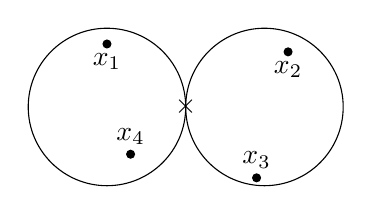
\begin{tikzpicture}
            \draw (-1, 0) circle (1);
            \draw (1, 0) circle (1);
            \node (0, 0) {$\times$};
            \draw[fill=black] (-1, 0.8) circle (0.05) node[below]{$x_1$};
            \draw[fill=black] (-0.7, -0.6) circle (0.05) node[above]{$x_4$};
            \draw[fill=black] (1.3, 0.7) circle (0.05) node[below]{$x_2$};
            \draw[fill=black] (0.9, -0.9) circle (0.05) node[above]{$x_3$};
        \end{tikzpicture}
    \end{gather*}
    From the point of view of $x_2$ and $x_3$ (the original coordinate chart), the marked points $x_1$ and $x_4$ have collapsed, while from the point of view of the latter (after the transformation $x\longrightarrow x/c$) the former have collapsed. This ``bubbling'' is what will generally happen at singular points. Curves that have this kind of singularity are called ``stable curves'':
    \newdef{Stable curve}{\index{stable!curve}\index{singularity!nodal}
        A compact, complex algebraic curve with $n$ marked points that satisfies the following conditions:
        \begin{enumerate}
            \item It has only simple \textbf{nodal singularities} (i.e.~singularities of the form $xy=0$).
            \item The marked points are distinct and do not coincide with the nodes.
            \item The curve has a finite number of automorphisms.
        \end{enumerate}
        One can \textbf{smoothen} a stable curve by replacing the neighbourhood of every node that consists of two disks by a cylinder. A stable curve can also be \textbf{normalized} by replacing these intersecting disks by disjoint disks.
    }
    \begin{remark}
        The last condition above is equivalent to requiring that every connected component of the normalization has negative Euler characteristic, i.e.~has itself a finite number of automorphisms.
    \end{remark}

    \begin{property}[Deligne-Mumford compactification]\index{Deligne-Mumford compactification}
        There exists a morphism of compact, complex orbifolds $\overline{\pi}:\overline{\mathcal{C}}_{g,n}\rightarrow\overline{\mathcal{M}}_{g,n}$ such that:
        \begin{itemize}
            \item $\mathcal{M}_{g,n}\subset\overline{\mathcal{M}}_{g,n}$ is a suborbifold with preimage $\mathcal{C}_{g,n}$ under $\overline{\pi}$,
            \item the fibres of $\overline{\pi}$ are stable curves of genus $g$ with $n$ marked points,
            \item each stable curve is isomorphic to a unique fibre, and
            \item the stabilizer of a point in $\overline{\mathcal{M}}_{g,n}$ is isomorphic to the automorphism group of the corresponding stable curve.
        \end{itemize}
    \end{property}

\subsection{Pseudoholomorphic maps}\label{section:stable_maps}

    \newdef{Cauchy-Riemann operator}{\index{Cauchy-Riemann!operator}
        Consider a complex vector bundle $(E,J)$ over an almost complex manifold $(M,j)$. A Cauchy-Riemann operator on $E$ is a complex-linear map
        \begin{gather}
            \mathrm{D}:\Gamma(E)\rightarrow\Gamma(\overline{\hom}(TM,E))
        \end{gather}
        satisfying the Leibniz rule
        \begin{gather}
            \mathrm{D}(f\sigma) = (\delbar f)\sigma + f(\mathrm{D}\sigma)\,,
        \end{gather}
        where $\overline{\hom}$ denotes the bundle of antilinear morphisms, i.e.~those vector bundle morphisms that anticommute with the almost complex structures.
    }
    This strongly resembles the definition of a Koszul connection \ref{bundle:koszul_connection}. The following property shows that this is no coincidence:
    \begin{property}
        For every Cauchy-Riemann operator $\mathrm{D}$ on a Hermitian vector bundle $(E,J)$ over an almost complex manifold $(M,j)$ there exists a Hermitian connection $\nabla$ such that
        \begin{gather}
            \mathrm{D}\sigma = \nabla\sigma + J\circ\nabla\sigma\circ j
        \end{gather}
        for all sections $\sigma\in\Gamma(E)$.
    \end{property}

    \newdef{Pseudoholomorphic function}{\index{pseudoholomorphic}\index{Cauchy-Riemann!conditions}
        Consider two almost complex manifolds $(M,J)$ and $(N,j)$. A function $f:(M,J)\rightarrow(N,j)$ is said to be pseudoholomorphic if it satisfies the \textbf{Cauchy-Riemann equations}
        \begin{gather}
            f_* + j\circ f_*\circ J = 0
        \end{gather}
        or, equivalently,
        \begin{gather}
            j\circ f_* = f_*\circ J\,,
        \end{gather}
        i.e.~the differential is complex-linear. This can rephrased in terms of a Cauchy-Riemann-like operator
        \begin{gather}
            \delbar_J:C^\infty(M,N)\rightarrow\Gamma(\overline{\hom}(TM,TM)):f\mapsto f_*+j\circ f_*\circ J\,,
        \end{gather}
        The kernel of this operator consists of exactly the pseudoholomorphic functions. Note that the image of $f$ under the above nonlinear Cauchy-Riemann operator is actually an element of $\Gamma(\overline{\hom}(TM,f^*TN))$, since the tangent space at a point $f\in C^\infty(M,N)$ is modelled on $\Gamma(f^*TN)$.\footnote{To make this statement precise one needs to endow $C^\infty(M,N)$ with the right topology, since this manifold is infinite-dimensional.} By Remark \ref{bundle:differential_remark} this operator can also be written in terms of the differential $\dr f$.
    }
    \begin{remark}[Pseudoholomorphic curves]
        In practice one often restricts to pseudoholomorphic curves, i.e.~pseudoholomorphic functions where the domain is a Riemann surface. On one hand in two dimensions one does not lose generality by only considering complex manifolds, since the integrability condition $\overline{\partial}^2=0$ is always satisfied. On the other hand, it is better to restrict to two-dimensional manifolds in the domain, because in general there are no nonconstant pseudoholomorphic functions (even locally) when the domain has a higher dimension.
    \end{remark}

    \begin{property}[Regularity]
        If a function of class $C^1$ satisfies the Cauchy-Riemann equations, it is automatically smooth.
    \end{property}

    \newdef{Pseudoholomorphic polygon}{
        For every polygon in $\mathbb{C}$, i.e.~a complex disk with a finite number of marked points, the Riemann mapping theorem gives a biholomorphism to the interior of the disk $D$. The \textit{Schwarz-Christoffel} formula gives an expression for this map, which can even be extended to the $n$-punctured disk $D_n$. A pseudoholomorphic $n$-gon in an almost complex manifold $M$ is a pseudoholomorphic map $f:D_n\rightarrow M$ such that $\lim_{w\rightarrow w_i}f(w)=q_i$, where $q_i$ is a vertex of the polygon and $w_i$ is a puncture of $D_n$.
    }

    \begin{property}[Symplectic submanifolds]
        Let $(M,\omega)$ be a symplectic manifold and consider an $\omega$-tame almost complex structure $J$. Every (complex) line in a tangent space is also a symplectic subspace. Globally, this means that every $J$-holomorphic curve corresponds to a symplectic submanifold.
    \end{property}

    \newdef{Energy}{\index{energy}
        Consider a symplectic manifold $(M,\omega)$ equipped with an $\omega$-tame almost complex structure $J$. By symmetrizing the form $\omega(\cdot,J\cdot)$ one obtains a (Riemannian) metric $g$. The energy of a $J$-holomorphic curve $f:(\Sigma,J_0)\rightarrow(M,J)$ is defined as follows:
        \begin{gather}
            \mathrm{E}(f) := \int_\Sigma f^*\omega = \frac{1}{2}\int_\Sigma \|\dr f\|^2\mathrm{Vol}_\Sigma.
        \end{gather}
        This quantity is always nonnegative and is zero if and only if $f$ is locally constant. (Note that for the second expression one needs the induced metric on both $\Sigma$ and $M$.)
    }

    \begin{construct}[Moduli space]
        Choose two integers $g,n\geq1$ and a homology class $A\in H_2(M)$. The moduli space $\mathcal{M}^A_{g,n}$ is defined as the set of equivalence classes of tuples $(\Sigma,J_0,f,z_1,\ldots,z_n)$, where $(\Sigma,J_0)$ is a Riemann surface of genus $g$, $f:(\Sigma,J_0)\rightarrow(M,J)$ is a pseudoholomorphic curve such that $f_*[\Sigma]=A$ and $\{z_i\}_{i\leq n}$ are marked points of $\Sigma$. Two such tuples are deemed equivalent if there exists an automorphism (i.e.~a biholomorphic or conformal diffeomorphism) that preserves the order of the marked points.
    \end{construct}
    \begin{example}
        When $M=\{\ast\}$, the moduli space reduces to $\mathcal{M}_{g,n}$, the moduli space of Riemann surfaces of genus $g$ with $n$ marked points.
    \end{example}

\section{Cohomology}
\subsection{Dolbeault cohomology}\index{Dolbeault!cohomology}

    \begin{theorem}[Hodge decomposition]\index{Hodge!decomposition}
        Let $M$ be a compact K\"ahler manifold.
        \begin{gather}
            H^k_\text{dR}(M)\cong\bigoplus_{p+q=k}H^{p,q}(M)
        \end{gather}
        for all $k\in\mathbb{N}$
    \end{theorem}

    By analogy with the Poincar\'e lemma for smooth manifolds one can prove the following theorems:
    \begin{theorem}[$\partial$-lemma]\index{$\partial$-lemma}
        Let $\alpha\in\Omega^{p,q}(M)$. If $\partial\alpha = 0$, locally there exists a complex form $\beta\in\Omega^{p-1,q}$ such that $\alpha = \partial\beta$.
    \end{theorem}
    \begin{theorem}[$\overline{\partial}$-lemma]
        Let $\alpha\in\Omega^{p,q}(M)$. If $\overline{\partial}\alpha = 0$, locally there exists a complex form $\beta\in\Omega^{p,q-1}$ such that $\alpha = \overline{\partial}\beta$.
    \end{theorem}
    \begin{theorem}[$\partial\overline{\partial}$-lemma]\label{complex:del_delbar_lemma}
        Let $\alpha\in\Omega^{p,q}(M)$. If $\dr\alpha = 0$, locally there exists a complex form $\beta\in\Omega^{p-1,q-1}$ such that $\alpha = \partial\overline{\partial}\beta$.
    \end{theorem}

\subsection{\difficult{Lagrangian Floer homology}}

    In this section a (co)homology theory is constructed from the intersection theory of Lagrangian submanifolds (see Chapter \ref{chapter:symplectic} for an introduction).

    Recall the pseudoholomorphic polygons from Section \ref{section:stable_maps}. In the study of symplectic manifolds, one often has a set of boundary conditions $\{L_i,q_i\}_{i\leq n}$, where the $L_i$ are Lagrangian submanifolds and the $q_i\in L_i\cap L_{i+1\bmod n}$ are intersection points. A pseudoholomorphic $n$-gon satisfies these boundary conditions if the edges of the domain are mapped to the submanifolds $L_i$ and the marked points to the intersection points $q_i$.

    \begin{property}[Moduli space]
        To fully appreciate Floer theory, one needs to study the moduli space of pseudoholomorphic polygons. One of the most important parts being compactness and the \textit{Gromov compactification}. For certain one-parameter families of polygons, the limit is a degenerate configuration that is not part of the moduli space itself. Consider for example the situation in Figure \ref{fig:floer_breaking}. The Lagrangian submanifolds are indicated by black lines (infinite straight lines are Lagrangian submanifolds of the complex plane). The interior of the polygon is sketched by a red line and the marked points are indicated by red dots.

        \begin{figure}[ht!]
            \centering
            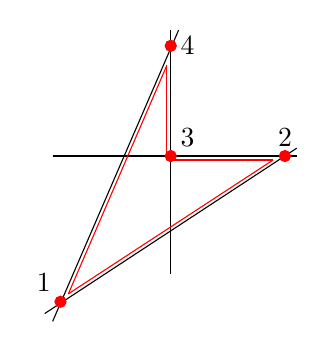
\begin{tikzpicture}
                \draw (0, 1.6) -- (0, -1.5);
                \draw (-1.5, 0) -- (1.6, 0);
                \draw (1.6, 0.1) -- (-1.6, -2);
                \draw (0.1, 1.6) -- (-1.5, -2.1);
                \draw[color = red] (-0.05, 1.15) -- (-0.05, -0.05);
                \draw[color = red] (-0.05, -0.05) -- (1.3, -0.05);
                \draw[color = red] (1.3, -0.05) -- (-1.3, -1.75);
                \draw[color = red] (-0.05, 1.15) -- (-1.3, -1.75);
                \node (3) at (0, 0) [above right]{3};
                \node (2) at (1.45, 0) [above]{2};
                \node (4) at (0, 1.4) [right]{4};
                \node (1) at (-1.4, -1.85) [above left]{1};
                \draw[fill = red, color = red] (1.45, 0) circle (2pt);
                \draw[fill = red, color = red] (0, 1.4) circle (2pt);
                \draw[fill = red, color = red] (0, 0) circle (2pt);
                \draw[fill = red, color = red] (-1.4, -1.85) circle (2pt);
            \end{tikzpicture}
            \caption{Pseudoholomorphic 4-gon.}
            \label{fig:floer_breaking}
        \end{figure}
        Now, one can make a one-parameter family of 4-gons that satisfies the same boundary conditions by, instead of going directly from vertex 3 to vertex 4, first going a bit down and then going up again, i.e.~making a ``slit''. This still satisfies all the properties to apply the Riemann mapping theorem, but gives a different polygon map. At a certain point a new vertex is created on the lower Lagrangian, a so-called \textbf{nodal} vertex, and the 4-gon is broken up into two 3-gons. From the domain point of view what happens is that two boundary punctures have collided and a new disk (with two punctures) has been attached. Adding such configurations to the moduli space to account for these limit operations gives rise to a \textit{Deligne-Mumford compactification}. Because finding all possible ways to arrange $n+1$ points on different attached disks (without altering their order) is equivalent to finding all possible parenthesations of $n+1$ symbols, one finds that the compactified moduli space of boundary-punctured disks $\overline{\mathcal{M}}_{n+1}$ is isomorphic to the $n^{th}$ Stasheff polytope $K_n$.

        In the case of bigons (for simplicity), three types of degeneracies can occur:
        \begin{itemize}
            \item\textbf{Strip breaking}: Here, energy concentrates at one of the marked points. There exists a sequence of bigons $\seq{f}$, here viewed as homotopies, and a diverging sequence of numbers $\seq{a}$ such that
            $\lim_{n\rightarrow\infty}f_n(s-a_n,t)$ is not the constant strip. This corresponds to the situation in Figure \ref{fig:floer_breaking}.
            \item\textbf{Disk bubbling}: Here, energy concentrates at a point on the boundary. There exists a sequence of bigons that can be rescaled such that the limit is a pseudoholomorphic disk entirely contained in one of the boundary Lagrangians.
            \item\textbf{Sphere bubbling}: Here energy concentrates at a point in the interior of a bigon. There exists a sequence of bigons that can be rescaled such that the limit is a pseudoholomorphic sphere entirely contained in the interior of $M$.
        \end{itemize}
        The latter two issues can be avoided by imposing topological restrictions such as by restricting to \textit{montone Lagrangian submanifolds} or by requiring that $[\omega]\cdot\pi_2(M,L)=0=[\omega]\cdot\pi_2(M,L')=0$.
    \end{property}

    \newdef{Floer complex}{
        Let $M$ be a symplectic manifold equipped. For every two transversally intersecting Lagrangian submanifolds, the chain group is defined as the free vector space generated by the intersection points: $C\!F(L,L') := \Lambda^{L\cap L'}$, where, to avoid technical difficulties, one should take the field $\Lambda$ to be a \textit{Novikov field}.

        The differential is defined by counting pseudoholomorphic bigons:
        \begin{gather}
            \partial\langle p\rangle := \sum_{q\in L\cap L'\backslash\{p\}}n(p,q)\langle q \rangle\,,
        \end{gather}
        where $n(p,q)$ denotes the number of (isomorphism classes of\footnote{The domain, i.e.~the disk with two boundary punctures, has as automorphism group $\mathbb{R}$. It scales the distance between the punctures.}) pseudoholomorphic bigons with boundary conditions $\{L,L',p,q\}$ of finite symplectic energy.
    }

    To be more precise, denote by $\mathcal{M}(p,q;[f])$ the moduli space of pseudoholomorphic bigons of finite symplectic energy in a fixed homotopy class $[f]\in\pi_2(M,L\cap L')$. The Maslov index of such a class can be defined using the spectral flow approach:
    \begin{gather}
        \mu([f]) := \mathrm{ind}(\mathrm{D}_{\delbar_J})\,,
    \end{gather}
    where $\mathrm{D}_{\delbar_j}$ denotes the linearization of the Cauchy-Riemann operator associated to $J$ (it can be shown that this operator is Fredholm and, hence, admits a well-defined index). When all bigons are regular, i.e.~when the linearized Cauchy-Riemann operator is surjective everywhere, the moduli space has dimension $\mu([f])-1$. Moreover, the \textit{Gromov compactness theorem} (see the property above) states that this manifold is compact.

    Putting a well-defined grading on $C\!F(L,L')$ is a bit more subtle. Let $\mathrm{LGr}(TM)$ denote the Lagrangian Grassmann bundle over $M$. The Maslov index of a bigon should only depend on the difference in degrees of its marked points and not on its homotopy class. This is implemented as follows (only a $\mathbb{Z}$-grading is considered here).
    \newdef{Maslov covering}{\index{Maslov!covering}
        A \textbf{Maslov covering} of $M$ is a $\mathbb{Z}$-covering $\mathcal{L}\rightarrow\mathrm{LGr}(TM)$ such that the fibre over every Lagrangian is given by the $\mathbb{Z}$-covering of $\mathrm{LGr}(\mathbb{R}^{\dim(M)})$. This corresponds to patching together the universal covers of the Lagrangian Grassmannians at every point of $M$.

        A Maslov covering exists if and only if the first Chern class is 2-torsion:
        \begin{gather}
            2c_1(M) = 0.
        \end{gather}
    }

    (This can be restated in cohomological conditions involving the Chern class \cite{moshayedi}: $c_1(M)$ should be 2-torsion and $\mu\in H^1$ should vanish for both $L$ and $L'$. This allows to lift a Lagrangian submanifold to a graded Lagrangian submanifold, a section of the universal cover of the Lagrangian Grassmann bundle.)
    \begin{gather}
        \partial\langle p \rangle = \sum_{\substack{q\in L\cap L'\\\mathrm{ind}([f])=1}}\big|\mathcal{M}(p,q;[f])\big|\,T^{\omega([f])}\langle q \rangle\,,
    \end{gather}
    where $T$ is the generator of the \textit{Novikov field} $\Lambda$ and $\omega([f])$ denotes the symplectic energy of $[f]$.

    \begin{property}[Hamiltonian isotopy]
        Consider two Lagrangian submanifolds $L,L'$. If there exists a Hamiltonian isotopy $L'\rightarrow L''$, then
        \begin{gather}
            H\!F(L,L')\cong H\!F(L,L'').
        \end{gather}
        If there exists a Hamiltonian isotopy $L\rightarrow L'$, then
        \begin{gather}
            H\!F(L,L')\cong H^\bullet(L)\,,
        \end{gather}
        where the left-hand side denotes singular cohomology.
    \end{property}

    \newdef{Symplectic action functional}{
        For every two Lagrangian submanifolds $L,L'\subset M$, one can consider the space of smooth paths connecting $L$ and $L'$:
        \begin{gather}
            \mathcal{P}(L,L') := \{\gamma\in C^1([0,1],M)\mid\gamma(0)\in L,\gamma(1)\in L'\}.
        \end{gather}
        The symplectic action functional is defined as follows:
        \begin{gather}
            A:\widetilde{\mathcal{P}}(L,L')\rightarrow\mathbb{R}:[\gamma,h]\mapsto\int_{[0,1]\times[0,1]}h^*\omega\,,
        \end{gather}
        where $\omega$ is the symplectic form on $M$ and $\widetilde{\mathcal{P}}$ denotes the universal cover (of a connected component) of $\mathcal{P}$, i.e.~the set of equivalence classes of pairs $(\gamma,h)$ where $h$ is a homotopy between $\gamma$ and a fixed point in the connected component.\footnote{To be correct one should use the so-called \textit{Novikov covering}.} If the symplectic form is trivialisable on $h$, Stokes's theorem implies that this integral is (up to a constant depending on the choice of base point) equal to
        \begin{gather}
            \int_{[0,1]}\gamma^*\theta\,,
        \end{gather}
        where $\theta$ is the symplectic potential.

        One can also calculate the differential of the action functional or, by introducing a (family of) compatible almost complex structure(s), the gradient of the action functional:
        \begin{gather}
            \mathrm{grad} A([\gamma,h])=J_t\pderiv{\gamma}{t}.
        \end{gather}
        It follows that the critical points of the functional correspond to constant paths, i.e.~intersection points of the Lagrangian submanifolds. Moreover, the flow equation of this gradient is exactly the Cauchy-Riemann equation of $J$-holomorphic curves with the given Lagrangian boundary conditions. In (finite-dimensional) Morse homology (Section \ref{section:morse}) one counts flow lines of the Hamiltonian flow, so it follows that one can interpret Lagrangian Floer homology as the infinite-dimensional analogue of Morse homology for the symplectic action functional.
    }

    \newdef{Fukaya category}{\index{Fukaya category}
        Consider a symplectic manifold $(M,\omega)$. The associated Fukaya category consists of the following data:
        \begin{enumerate}
            \item\textbf{Objects}: Lagrangian submanifolds of $M$.
            \item\textbf{Morphisms}: When $L\pitchfork L'$, $\hom(L,L'):=C\!F(L,L')$, the (Lagrangian) Floer chain group.
        \end{enumerate}
        This definition can be generalized to obtain an $A_\infty$-category. Whenever the Lagrangian submanifolds intersect transversally, a multiplication map
        \begin{gather}
            \mu:\hom(L',L'')\otimes\hom(L,L')\rightarrow\hom(L,L'')
        \end{gather}
        can be defined. Consider intersection points $q_1\in L\cap L',q_2\in L'\cap L''$ and $q\in L\cap L''$. The coefficient of $q$ in $\mu(q_2,q_1)$ is obtained by counting pseudo-holomorphic 3-gons with boundary on the Lagrangians and marked points $q_1,q_2$ and $q$.
    }
    \begin{remark}[Bubbles]\index{bubble}
        Aside from breaking and splitting of holomorphic polygons, another situation where degenerate polygons arise is the so-called bubbling phenomenon, where a holomorphic sphere (0-gon) pops up. Unless the symplectic manifold and the boundary Lagrangian are exact, these give rise to a ``vacuum constant'' in the sense that the $A_\infty$-structure is modified to a curved $A_\infty$-structure with $m_0\neq 0$.
    \end{remark}

    ?? COMPLETE ??